% Copyright (c)  2005-2010 EDF-EADS-PHIMECA.
% Permission is granted to copy, distribute and/or modify this document
% under the terms of the GNU Free Documentation License, Version 1.2
% or any later version published by the Free Software Foundation;
% with no Invariant Sections, no Front-Cover Texts, and no Back-Cover
% Texts.  A copy of the license is included in the section entitled "GNU
% Free Documentation License".
\renewcommand{\etapemethodo}{B}
\renewcommand{\nomfichier}{docref_B122_Copulas}
\renewcommand{\titrefiche}{Copula}

\Header

\MathematicalDescription{

  \underline{\textbf{Goal}}\\

  To define the joined probability density function of the random input vector $\uX$ by composition, one needs:
  \begin{itemize}
  \item the specification of the copula of interest $C$ with its parameters,
  \item the specification of the ${n_X}$ marginal laws of interest $F_{X_i}$ of the ${n_X}$ input variables $X_i$.
  \end{itemize}

  The joined cumulative density function is therefore defined by :
  $$
  \mathbb P\left( X^1 \leq x^1, X^2 \leq x^2, \cdots, X^{n_X} \leq x^{n_X}\right)       = C\left(F_{X^1}(x^1),F_{X^2}(x^2),\cdots,F_{X^{n_X}}(x^{n_X}) \right)
  $$

  Within this part, we define the concept of copula and its use within Open TURNS.\\


  \underline{\textbf{Principles}}\\

  The copulas enable to represent the part of the joined cumulative density function which is not described by the marginal laws. It enables to represent the dependence structure of the input variables. A copula is a special cumulative density function defined on $[0,1]^{n_X}$ whose marginal distributions are uniform on $[0,1]$. The choice of the dependence structure is disconnected from the choice of the marginal distributions.\\

  \underline{\textbf{Basic properties of copulas}}\\

  A copula, restricted to $[0,1]^{n_X}$ is a $n_U$-dimensional cumulative density function with uniform marginals.

  \begin{itemize}
  \item $C(\underline{u}) \geq 0$,  $\forall \underline{u} \in [0,1]^{n_U}$
  \item $C(\underline{u}) = u_i$, $\forall \underline{u}=(1,\ldots,1,u_i,1,\ldots,1)$
  \item For all $N$-box $\mathcal B = [a_1,b_1] \times \cdots \times [a_{n_U},b_{n_U}] \in [0,1]^{n_U}$, we have $\mathcal V_C(\mathcal B) \geq 0$,     where:
    \begin{itemize}
    \item       $\mathcal V_C(\mathcal B) = \sum_{i=1,\cdots, 2^{n_U}} sign(\underline{v}_i) \times C(\underline{v}_i)$, the summation being made over the $2^{n_U}$ vertices $\underline{v_i}$ of $\mathcal B$.
    \item       $sign(\underline{v}_i)= +1$ if $v_i^k = a_k$ \textit{for an even number of} $k's$, $sign(\underline{v}_i)= -1$ \textit{otherwise}.\\
    \end{itemize}
  \end{itemize}

  \underline{\textbf{Copulas available within Open TURNS}}\\

  Different copulas are available within Open TURNS:\\

  {\bf Independent Copula}: It means that all the input variables are independent the ones from the others. The independent copula is defined by:
  $$
  C^{Indep}(u_1,u_2,\cdots,u_{n_{\:U}}) = \prod_{i=1}^{n_{\:U}} u_i
  $$

  {\bf Gaussian Copula}: The Gaussian copula is parameterized by a correlation matrix $\mathbf R$. The Gaussian copula is thus defined by:
  $$
  C^{Gauss}_{\mathbf R} = \Phi_{\mathbf R}^{n_{\:U}}\left(\Phi^{-1}(u_1),\Phi^{-1}(u_2),\cdots,\Phi^{-1}(u_{n_{\:U}}) \right)
  $$
  where:
  \begin{itemize}
  \item $\Phi_{\mathbf R}^{n_{X}}$ is the multinormal cumulative density function in dimension ${n_{X}}$:
    $$
    \Phi_{\mathbf R}^{n_{X}}(\underline{x}) =  \int_{-\infty}^{x_1} \ldots \int_{-\infty}^{x_{n_{X}}} \frac{1}{{(2\pi.\det{\mathbf R})}^{\frac{n_{X}}{2}}} \: . \: e^{-\frac{^t\underline{u}.\mathbf R.\underline{u}}{2}} \: du_1\ldots du_{n_{\:X}}
    $$
  \item $\Phi$ is the cumulative distribution function of the normal law in dimension 1:
    $$
    \Phi(x) = \int_{-\infty}^x \frac{1}{\sqrt{2\pi}} \: e^{-\frac{t^2}{2}} \: dt
    $$
  \item $\mathbf R$ is the correlation matrix. This matrix is defined by its algebric properties: symmetric, definite and positive. \\
  \end{itemize}


  The correlation matrix $\mathbf R$ can be obtained by different means:
  \begin{itemize}
  \item If one knows the Spearmann correlation Matrix, that is to say,
    $$
    \rho_{ij}^S = \rho^S(X_i,X_j) = \rho^P(F_{X_i}(X_i),F_{X_j}(X_j))
    $$
    the correlation matrix $\mathbf R$ is deduced by the following formula:
    $$
    \mathbf R_{ij} = 2 \sin(\frac{\pi}{6}\rho_{ij}^S)
    $$
  \item If one knows the Kendall measure of correlation, that is to say,
    $$
    \tau_{ij} = \tau(X_i,X_j) = \mathbb P\left((X_{i_1} - X_{i_2}).(X_{j_1} - X_{j_2}) > 0 \right) - P\left((X_{i_1} - X_{i_2}).(X_{j_1} - X_{j_2}) < 0 \right)
    $$
    where $(X_{i_1},X_{j_1})$ and $(X_{i_2},X_{j_2})$ follow the law of $(X_i,X_j)$,
    the correlation matrix $\mathbf R$ is deduced by the following formula:
    $$
    \mathbf R_{ij} = \sin(\frac{\pi}{2} . \tau_{ij})
    $$
  \item If one knows the Pearson correlation Matrix $\mathbf R^P$, there are two possibilities:
    \begin{enumerate}
    \item       If and only if all the marginal laws are Gaussian,
      $$
      \mathbf R \equiv \mathbf R^P
      $$
    \item
      In the other cases, one has to build the correlation matrix $\mathbf R$ by inversion of the following formula from the Pearson Correlation Matrix $\mathbf R^P$:
      $$
      \mathbf R_{ij}^P = \int \int_{\mathbb R^2} (x^i-\mathbb E[X^i])(x^j-\mathbb E[X^j]) \Phi_{ij}(x^i,x^j,\mathbf R_{ij})dx^i dx^j
      $$
    \end{enumerate}
  \end{itemize}



  {\bf Frank Copula}: The Frank copula is parameterized by a scalar $\theta \neq 0 $  . The Frank copula is thus defined by:
  $$
  \displaystyle -\frac{1}{\theta}\log\left(1+\frac{(e^{-\theta u_1}-1)(e^{-\theta u_2}-1}{e^{-\theta}-1}\right)
  $$


  {\bf Clayton Copula}: The Clayton copula is parameterized by a scalar $\theta \geq 0 $ . The Clayton copula is thus defined by:
  $$
  \displaystyle \left(u_1^{-\theta}+u_2^{-\theta}-1\right)^{-1/\theta}
  $$


  {\bf Gumbel Copula}: The Gumbel copula is parameterized by a scalar $\theta \geq 0 $ . The Gumbel copula is thus defined by:
  $$
  \displaystyle \exp\left(-\left((-\log(u_1))^{\theta}+(-\log(u_2))^{\theta}\right)^{1/\theta}\right)
  $$

  {\bf Sklar Copula}: The Sklar copula is obtained directly from the expression of the $n$-dimensional distribution which cumulative distribution function is $F$ with $F_i$ its marginals :
  $$
  C(u_1, \dots, u_n) = F(F_1^{-1}(u_1), \dots, F_n^{-1}(u_n))
  $$


  {\bf Composed Copula}:
  A copula may be defined as the product of other copulas : if $C_1$ and $C_2$ are two copulas respectively of random vectors in  $\mathbb{R}^{n_1}$ and $\mathbb{R}^{n_2}$, we can create the copula of a random vector of $\mathbb{R}^{n_1+n_2}$, noted $C$ as follows :
  $$
  C(u_1, \cdots, u_n) = C_1(u_1, \cdots, u_{n_1}) C_2(u_{n_1+1}, \cdots, u_{n_1+n_2})
  $$
  It means that both subvectors $(u_1, \cdots, u_{n_1})$ and $(u_{n_1+1}, \cdots, u_{n_1+n_2})$ of $\mathbb{R}^{n_1}$ and $\mathbb{R}^{n_2}$ are independent.

}

{

}

\Methodology{
  This method of modelling the dependencies between the input variables is part of the step B of the global methodology ("quantify sources of uncertainty"). It enables to build an expression of the probability density function of the input variables $\uX$ defined in step A ("specification of the model and criteria") by composition with the marginal distributions of each $X^i$. This method requires the knowledge of the Spearman correlation matrix or the Kendall correlation measure. It can also be used if one knows the Pearson correlation matrix, but only with the assumption of Gaussian marginal laws for all the input variables. \\

}
{
  One has to pay attention that the composition of the marginal distributions and the copulas available in Open TURNS is not sufficient to represent all types of dependencies (see examples in the next section). Previous statistical and/or justifications should be done to justify this choice of modeling  dependencies. Besides, as previously discussed, the use of Copula is totally decoupled from the knowledge of the marginal laws of the input variables.

  The following references give a first entry point to the Copulas:
  \begin{itemize}
  \item Nelsen, 'Introduction to Copulas'

  \item Embrechts P., Lindskog F., Mc Neil A., 'Modelling dependence with copulas and application to Risk Management', ETZH 2001.

  \end{itemize}
}

\Example{

  Hereafter  are the iso-curves of the PDF respectively of some copulas of type : independent, Normal, Clayton, Gumbel, Frank.


  \begin{center}
    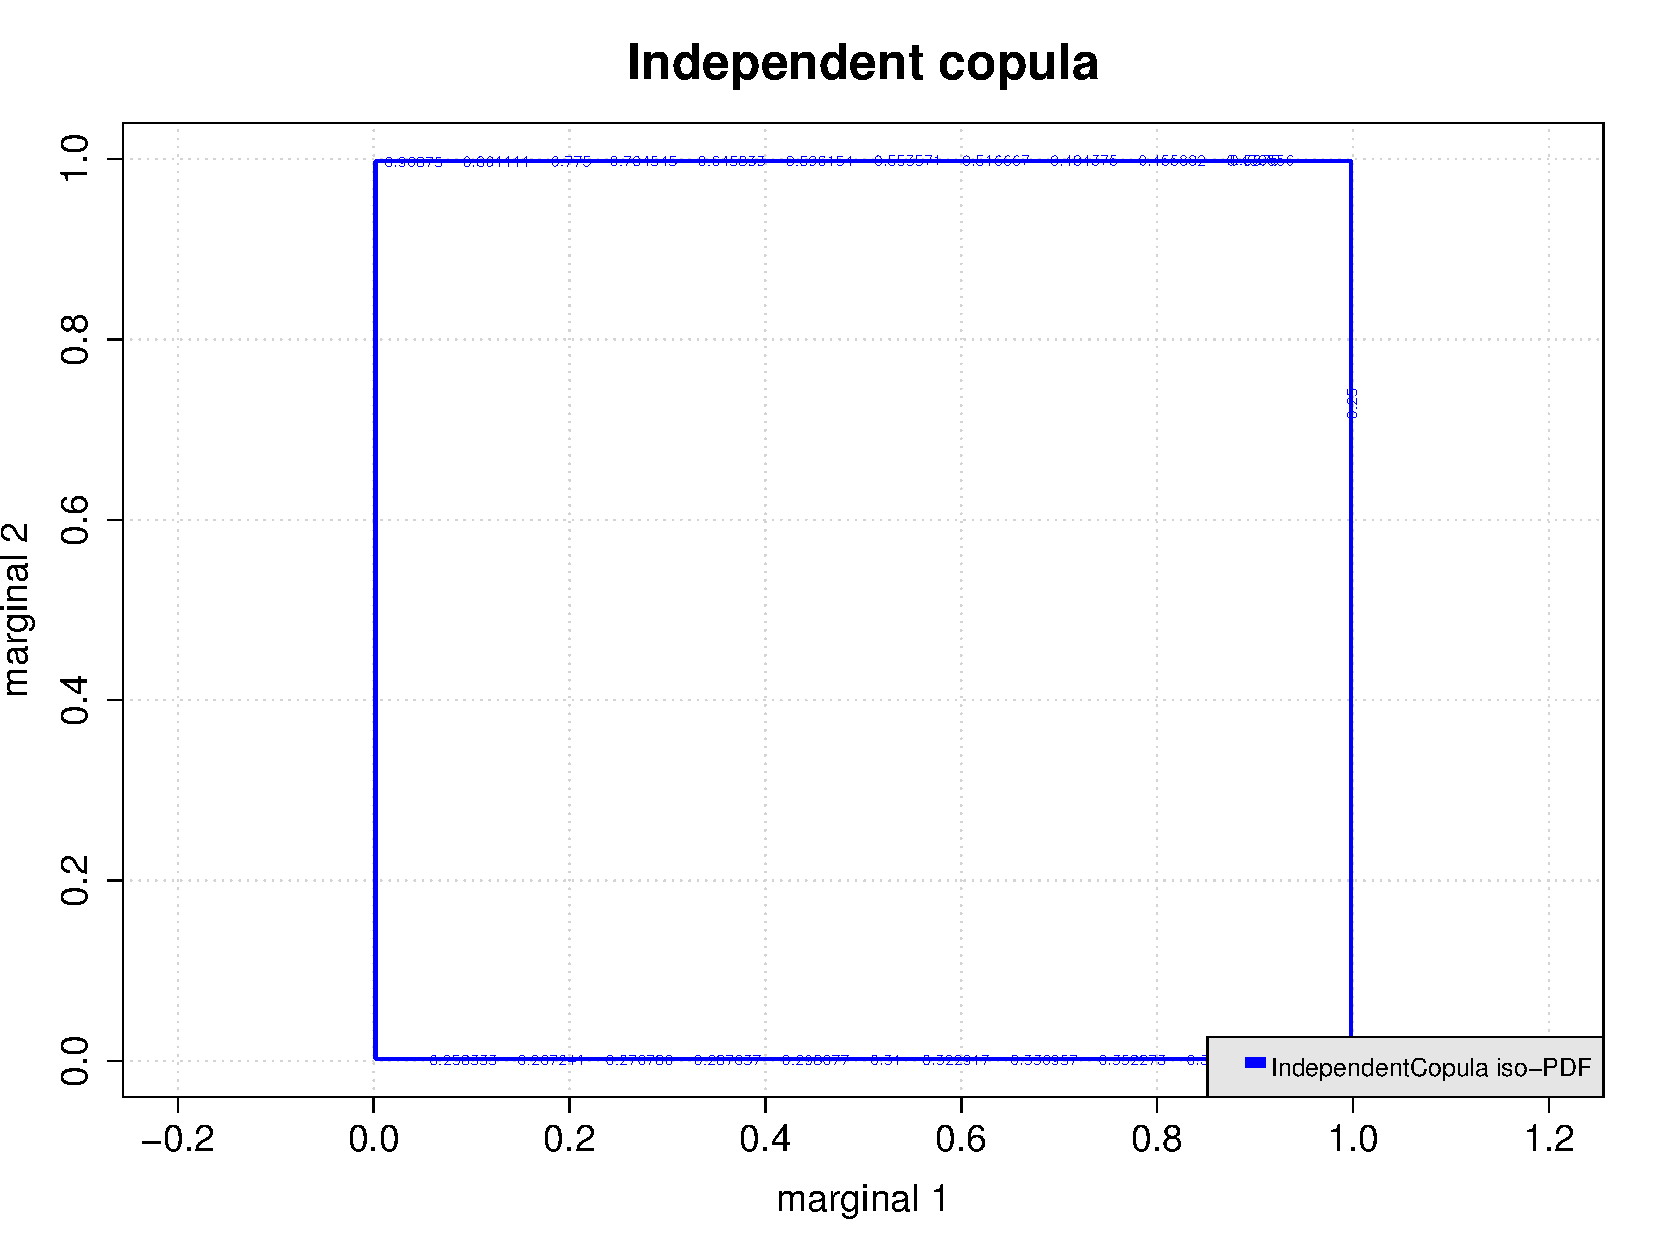
\includegraphics[width=7cm]{IndependentCopula.pdf}
  \end{center}


  \begin{center}
    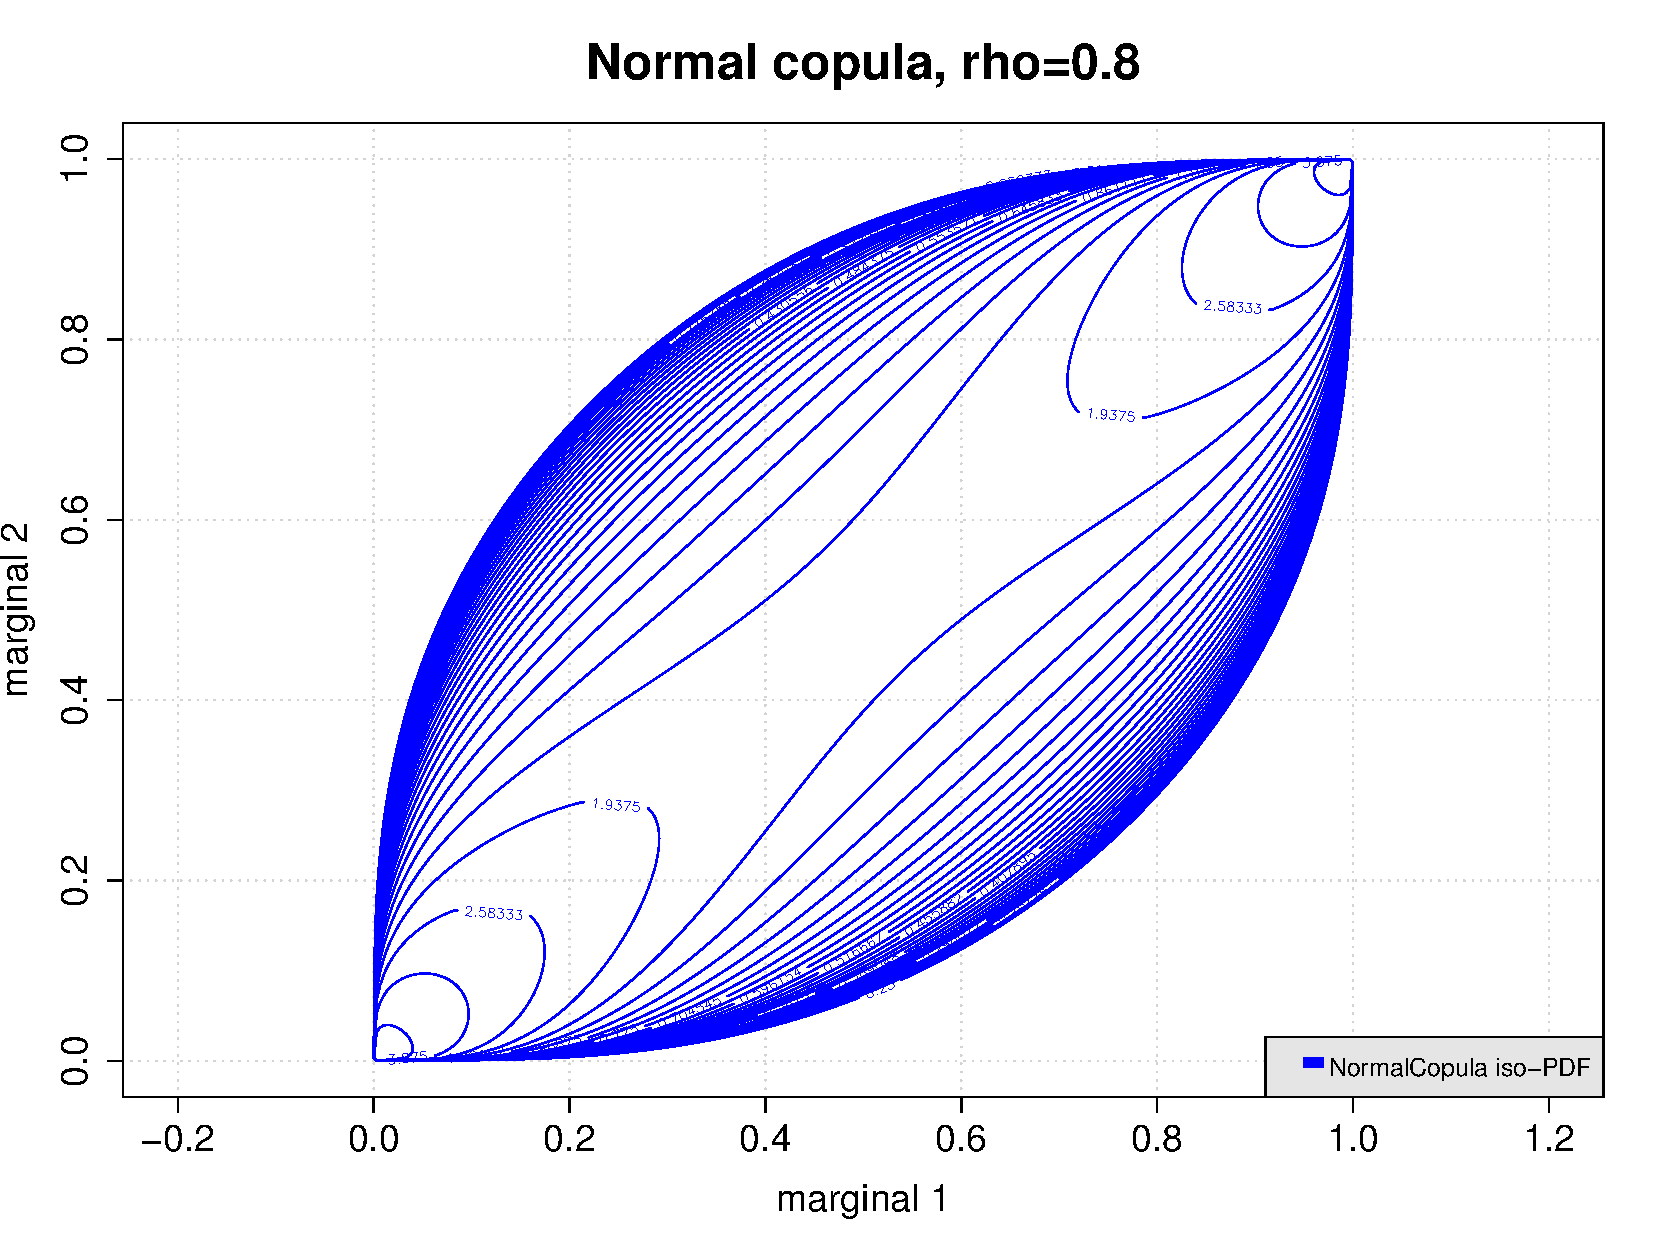
\includegraphics[width=7cm]{NormalCopula.pdf}
  \end{center}


  \begin{center}
    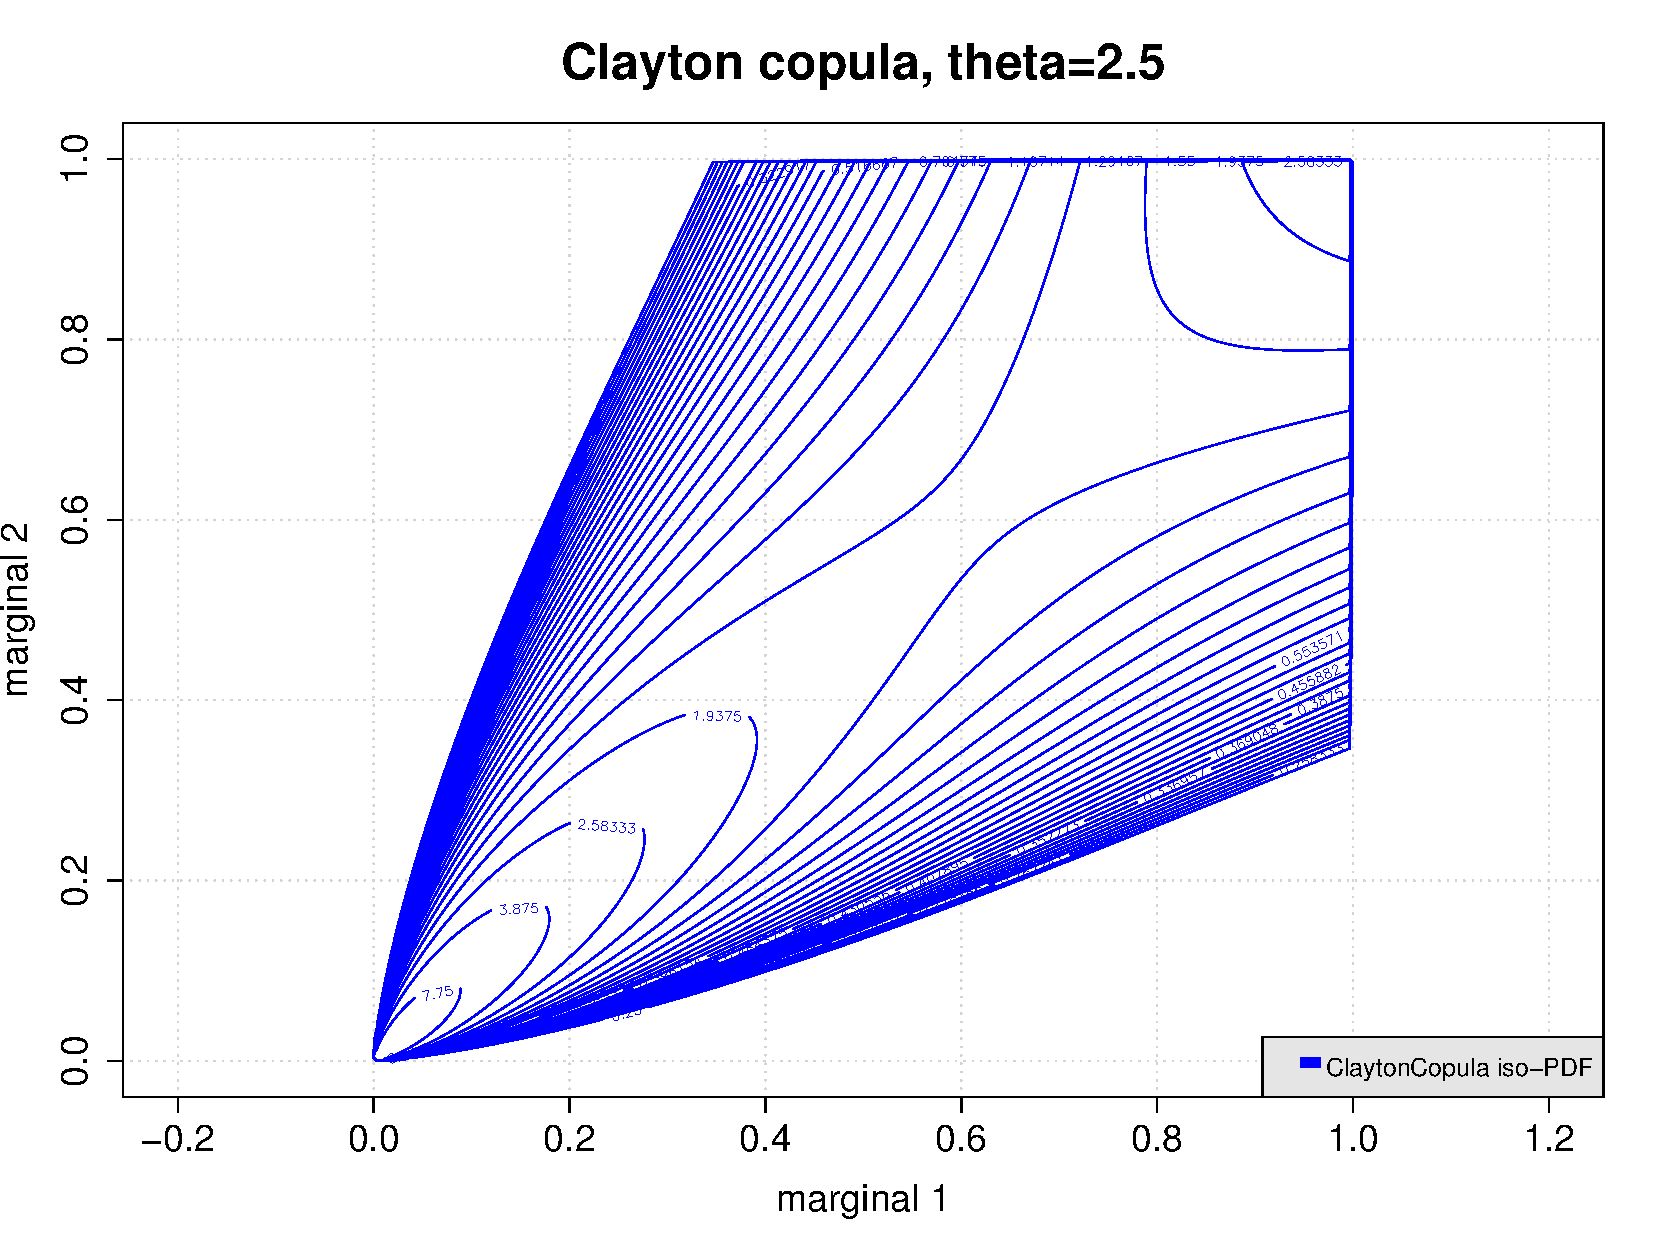
\includegraphics[width=7cm]{ClaytonCopula.pdf}
  \end{center}


  \begin{center}
    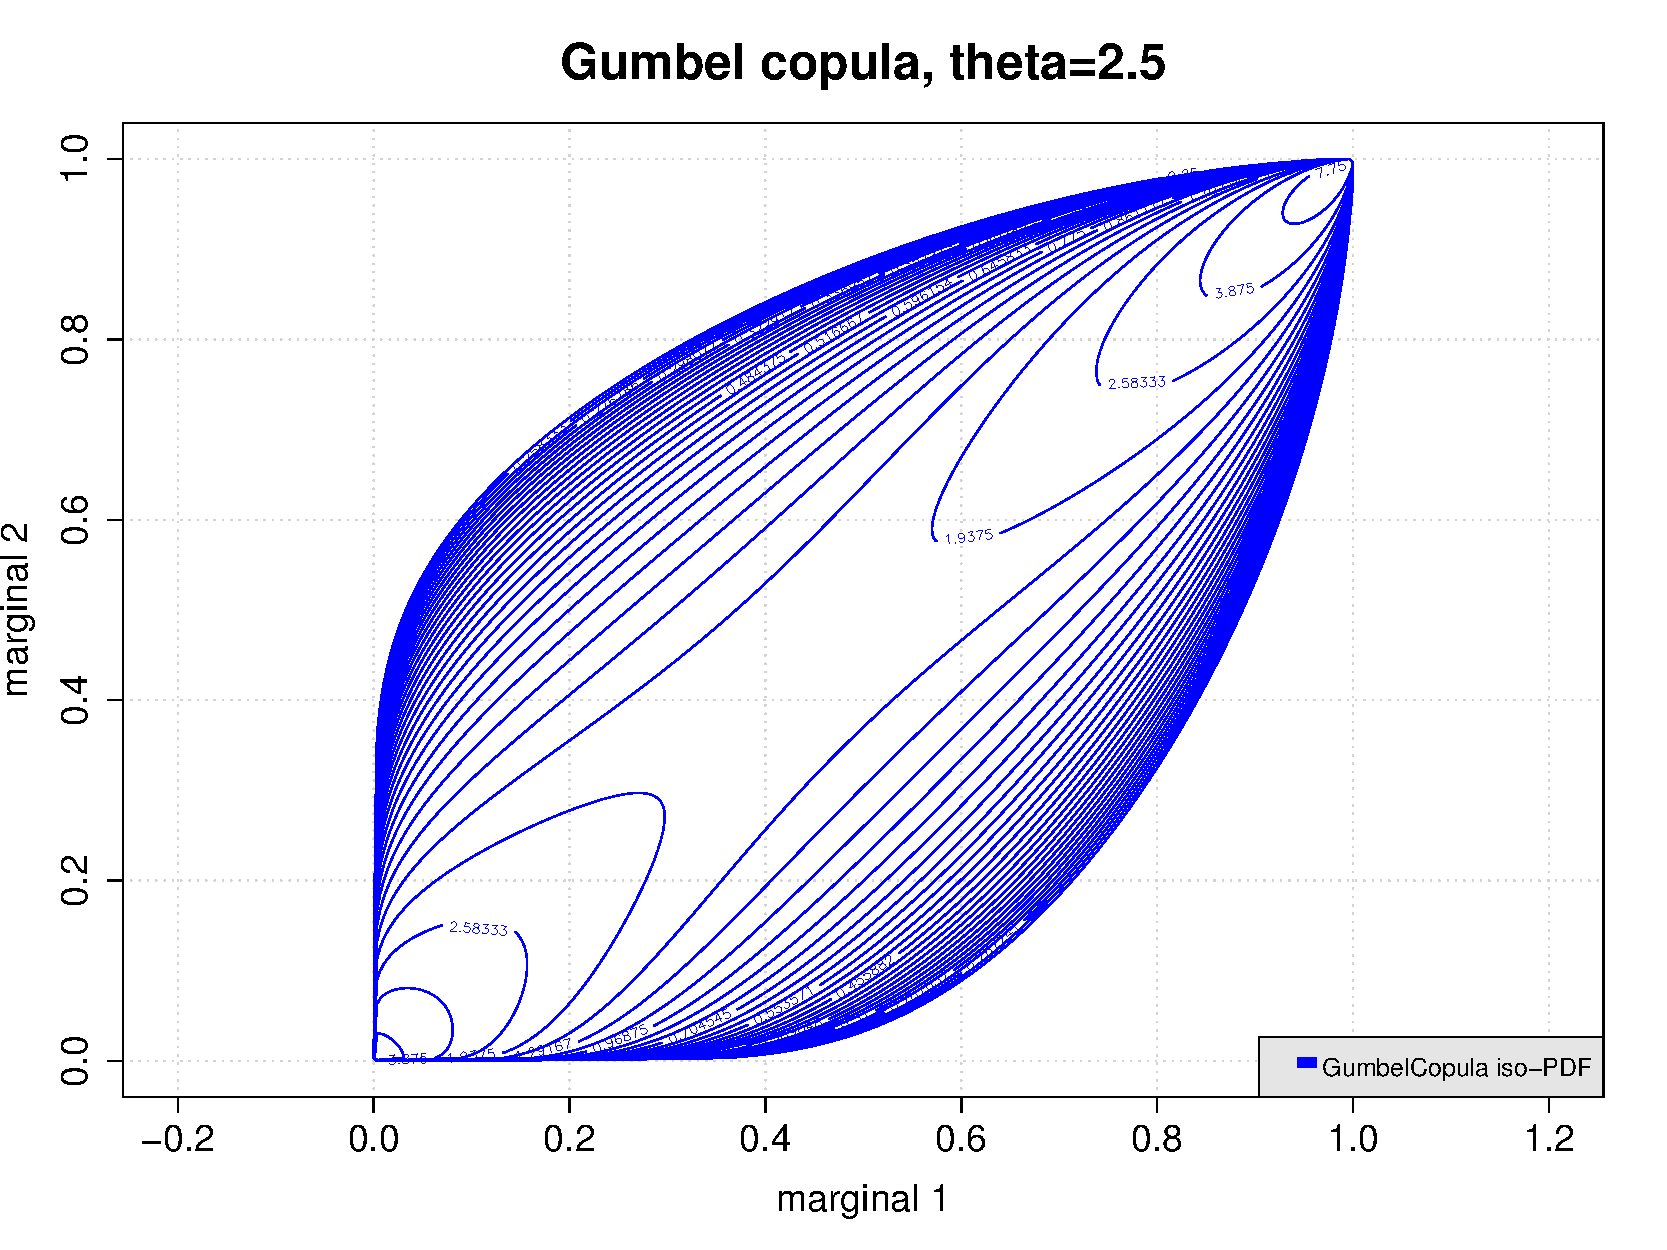
\includegraphics[width=7cm]{GumbelCopula.pdf}
  \end{center}

  \begin{center}
    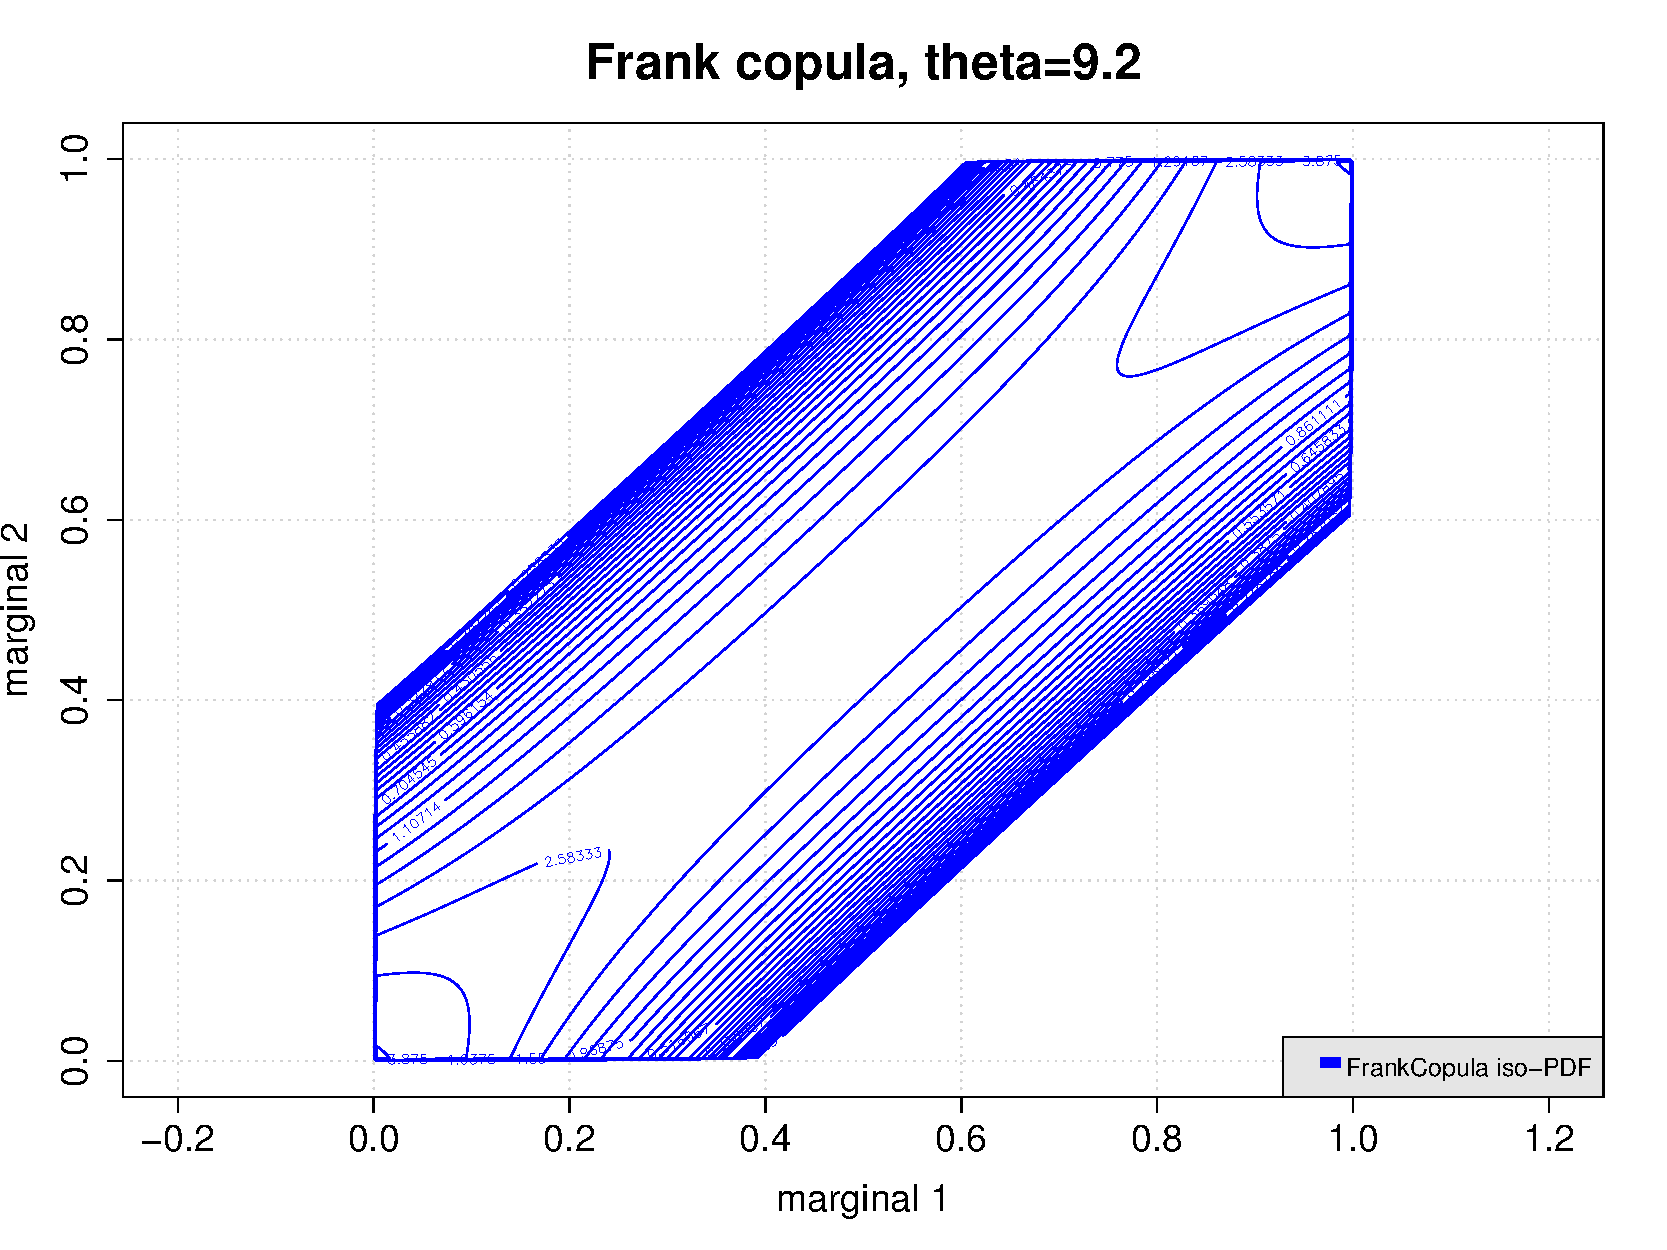
\includegraphics[width=7cm]{FrankCopula.pdf}
  \end{center}

}
